%!TEX root = ../template.tex
%%%%%%%%%%%%%%%%%%%%%%%%%%%%%%%%%%%%%%%%%%%%%%%%%%%%%%%%%%%%%%%%%%%%
%% chapter2.tex
%% NOVA thesis document file
%%
%% Chapter with the template manual
%%%%%%%%%%%%%%%%%%%%%%%%%%%%%%%%%%%%%%%%%%%%%%%%%%%%%%%%%%%%%%%%%%%%

\typeout{NT FILE chapter2.tex}

% \printbibliography[heading=subbibliography, segment=\therefsegment, title={\bibname\ for chapter~\thechapter}]
\glsresetall
\chapter{State of the Art}\label{cha:II_SotA}
% escrever aqui qlq coisa de introduçao:

\section{Global Navigation Satellite System}\label{II_gnss}

%MUDAR, ESTÁ COPIADO!
So, the difference between RTK and DGPS is that DGPS is the traditional differential GPS.
RTK is a specific type of DGPS.
but it uses a newer technology than the traditional DGPS.
RTK stands for real-time kinematic and commonly uses the RTCM protocol.
The traditional DGPS uses an older antiquated protocol while RTK uses a newer algorithm, and the protocol is based on RTCM3. 
%____________

Nowadays, whenever someone wishes to know their current location on Earth, just a few, effortless taps on a smartphone will be enough; this is often associated with GPS, which has been around for many years. In a more general manner, this technology can be described as a Global Navigation Satellite System, or GNSS. This term refers to any satellite constellation that can be used to help navigate throughout the world (as the name suggests). derives from a set of artificial satellites that comprises a network, and such network belongs 

to the average smartphone nowadays works as a GNSS receiver.
global navigation satellite system comprises a network of satellites that continuously orbit the Earth, constantly emmiting radio-frequecy (hyphen?) signals carrying information about their current status, position in space and precise time.
This information is acheived through atomic clocks, installed within the satellite itself.

smartphone = single-band ou multi-band?
how many constellations;
how many satellites in each constellation;

\section{RTK}\label{II_rtk}

\section{NTRIP}\label{sec:II_ntrip}

\section{Battery System}\label{sec:II_battery}
The formula is (Wh)/(h) = (W). For example, if you have 100 Wh for a duration of 2 hours, then the wattage is (100)/(2) = (50) Watts.
(Watthours is a measure of energy and watts is a unit of power. Power multiplied by time is enery).

como cada uma das baterias atualmente em uso is rated for (as?) 7.4V, 1070 mAh, that corresponds to 7.918 Wh.

% LiFePO$_4$ better than Li-ion batteries?
``The LiFePO$_4$ battery has the edge over lithium-ion, both in terms of cycle life (it lasts 4-5x longer), and safety. This is a key advantage because lithium ion batteries can overheat and even catch fire, while LiFePO4 does not''% citation needed

\subsection{USB Type-C}\label{sec:II_usb_c}
% ler wiki do USB-C e derivar os topicos daí
% depois ir ao IEEEXplore procurar papers que dêem backup
\subsubsection{Power Delivery}\label{sec:II_usb_c_PD}
% PD is a protocol

\section{Current Solutions}\label{sec:II_curr_solutions}

% \begin{tabularx}

% \end{tabularx}

\begin{table}[ht]       % provavelmente devo meter as palavras "parameter"/"base station" na caption?
	\centering          % ou devo eliminar a celula toda?
    \captionsetup{justification=centering}
    \caption{Compilation of the most relevant solutions available in the market (as of the date of the present document).}
	\label{tab:current_solutions_1}
	\begin{tabular}{|c|c|c|c|c|c|} % 8 colunas
		\toprule
		
        {} & {} & {} & \vtop{\hbox{\strut \textbf{beRTK}}\hbox{\strut \textbf{(Beyond Vision)}}} & \vtop{\hbox{\strut \textbf{Reach RS2}}\hbox{\strut \textbf{(Emlid)}}} & \vtop{\hbox{\strut \textbf{D-RTK 2}}\hbox{\strut \textbf{(DJI)}}}\\        
        
        \midrule

        \multirow{8}{*}{\rotatebox{90}{\textbf{Positioning}}}&\textbf{CorrectionT}\\
        &\multirow{5}{*}{\rotatebox{90}{\textbf{SupportedC}}}&\textbf{GPS}\\
        &\textbf{GLONASS}\\
        &X\\
        &X\\
        &X\\
        &X\\
        &X\\
        \midrule
        
        \rotatebox{90}{\textbf{Connectivity}} & 2 & 2 & 2 & 2 & 2\\
        \midrule

        \multirow{2}{*}{Multirow}&X\\
        &X & t\\

        \midrule\addlinespace[1.5ex]
        
        {} & 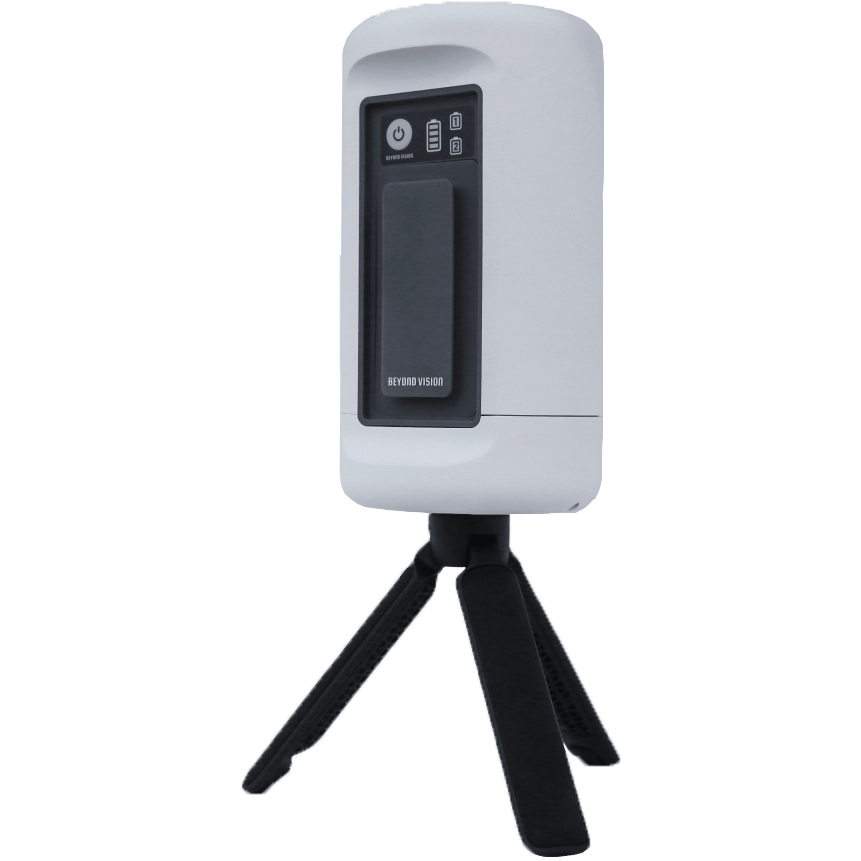
\includegraphics[height=1.4cm]{Chapters/Figures/base_stations/beRTK_2.png} & 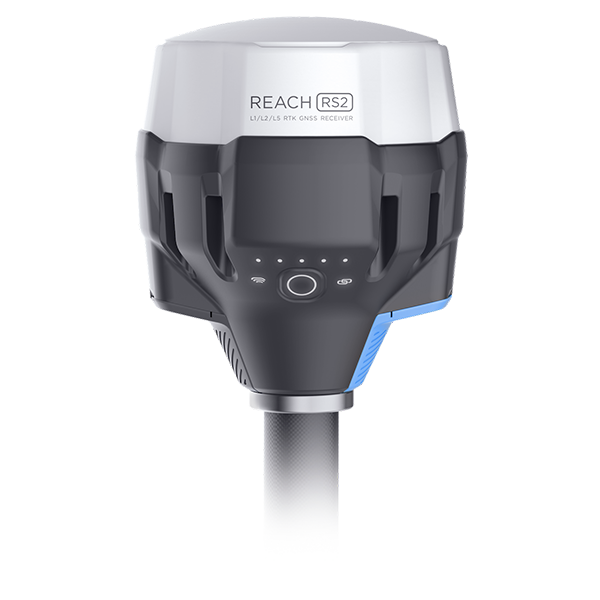
\includegraphics[height=1.4cm]{Chapters/Figures/base_stations/REACH-RS2.png} & 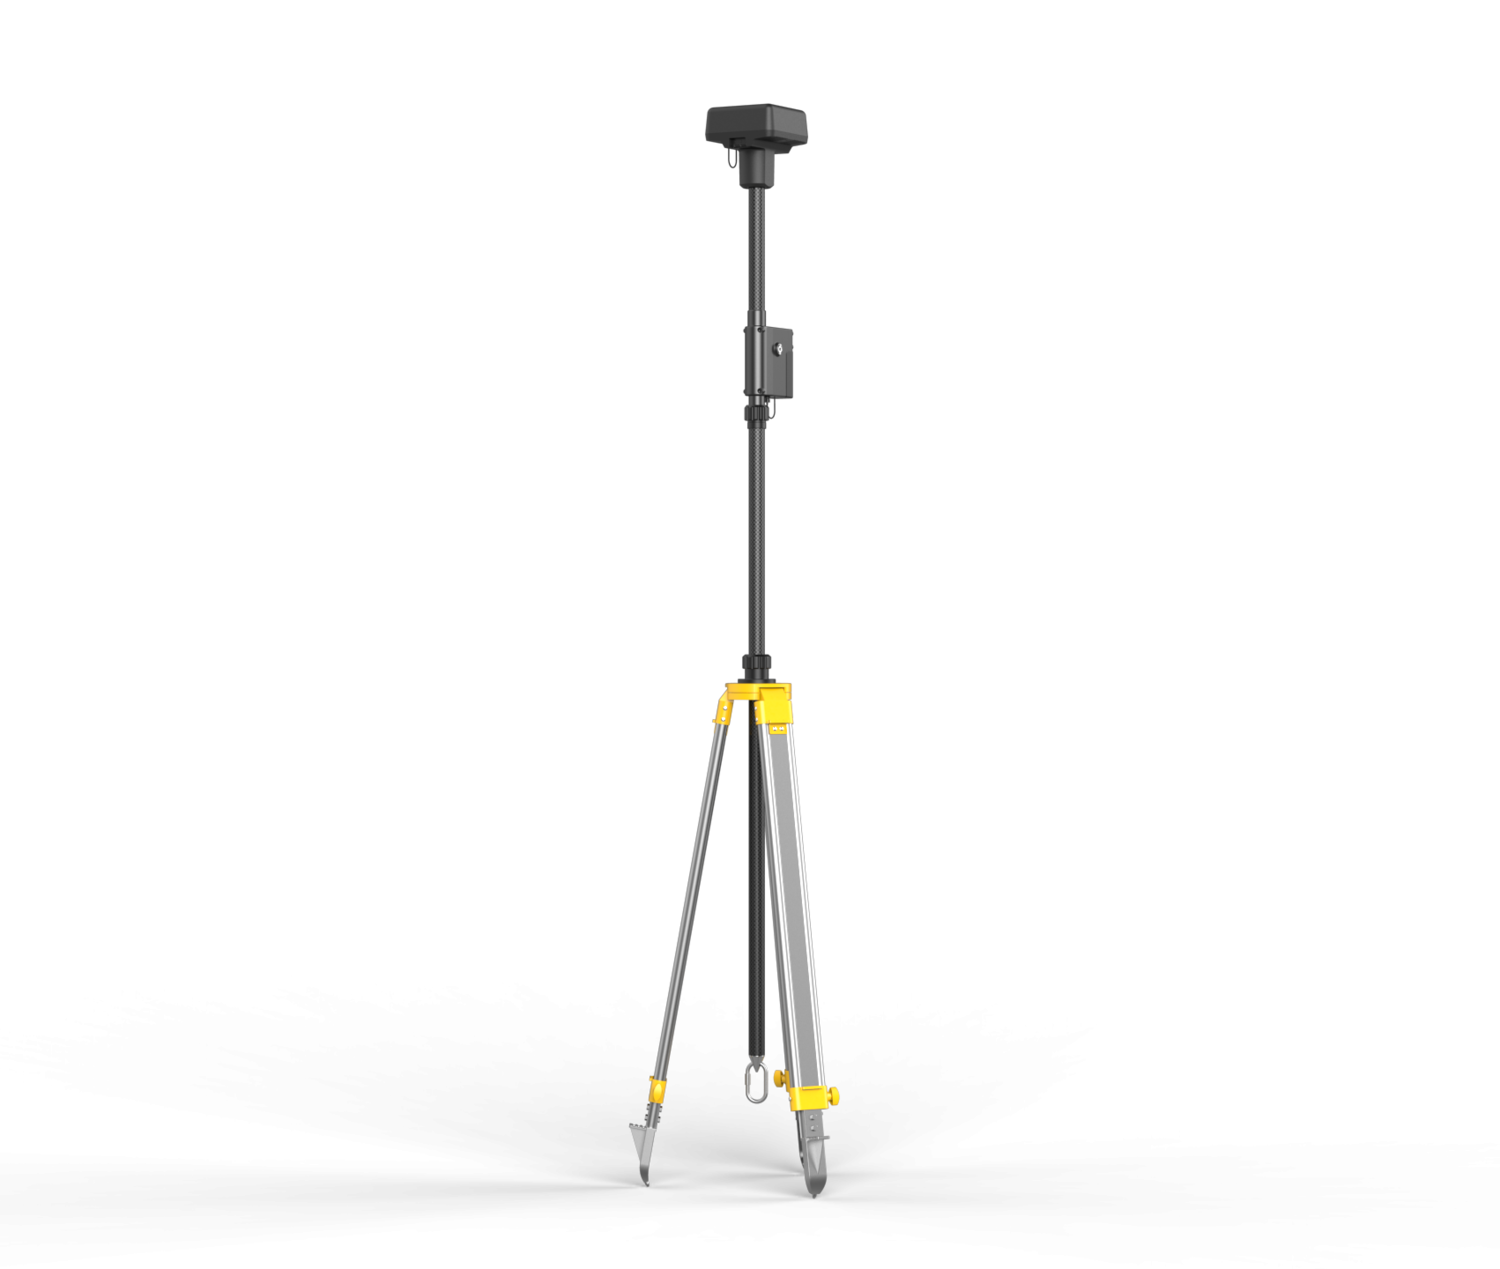
\includegraphics[height=1.4cm]{Chapters/Figures/base_stations/d-rtk-2.png}\\
		
        \bottomrule
        
	\end{tabular}
\end{table}

% tabela como multirow dento de multirow:
% \multirow{6}{*}{W2} & \multirow{3}{*}{3} & $0.090475\pm 0.011115$ & \multirow{3}{*}{21} & \multirow{3}{*}{6} & \multirow{3}{*}{3} \\
                    % &                    & $0.14861\pm 0.03562$   &                     &                    &                    \\
                    % &                    & $0.1861 \pm 0.01728$   &                     &                    &                    \\
                    % & 6                  & 8                      & 14                  & 5                  & 2                  \\
                    % & 9                  & 8                      & 14                  & 5                  & 2                  \\
                    % & 12                 & 8                      & 14                  & 5                  & 2                  \\


\begin{table}[ht]
    \centering
    \captionsetup{justification=centering}
    \caption{Compilation of the most relevant solutions available in the market (as of the date of the present document).}
	\label{tab:curr_solutions_positioning}
    \begin{tabular}{cccccccc} % 8 colunas
		\toprule
        \multicolumn{8}{c}{\textbf{Positioning}}\\
        \textbf{CorrectionT} &.
		\multicolumn{5}{c}{\textbf{SupportedC}}\\
        \textbf{GPS}&   \textbf{GLONASS}   &   \textbf{Galileo}   &   \textbf{BeiDou}   &   \textbf{NavIC}\\
        \bottomrule
	\end{tabular}
\end{table}



\begin{table}[ht]       % provavelmente devo meter as palavras "parameter"/"base station" na caption?
	\centering          % ou devo eliminar a celula toda?
    \captionsetup{justification=centering}
    \caption{Compilation of the most relevant solutions available in the market (as of the date of the present document).}
	\label{tab:current_solutions_2}
	\begin{tabular}{|c|c|c|c|c|} % 8 colunas
		\toprule
		{} & {} & {} & \vtop{\hbox{\strut \textbf{HiPer V}}\hbox{\strut \textbf{(Topcon)}}} & \vtop{\hbox{\strut \textbf{S990A GNSS Receiver}}\hbox{\strut \textbf{(Stonex)}}}\\        
        \midrule
        \rotatebox{90}{\textbf{pizza}} & 2 & 2 & 2 & 2\\
        \midrule\addlinespace[1.5ex]
        {} & 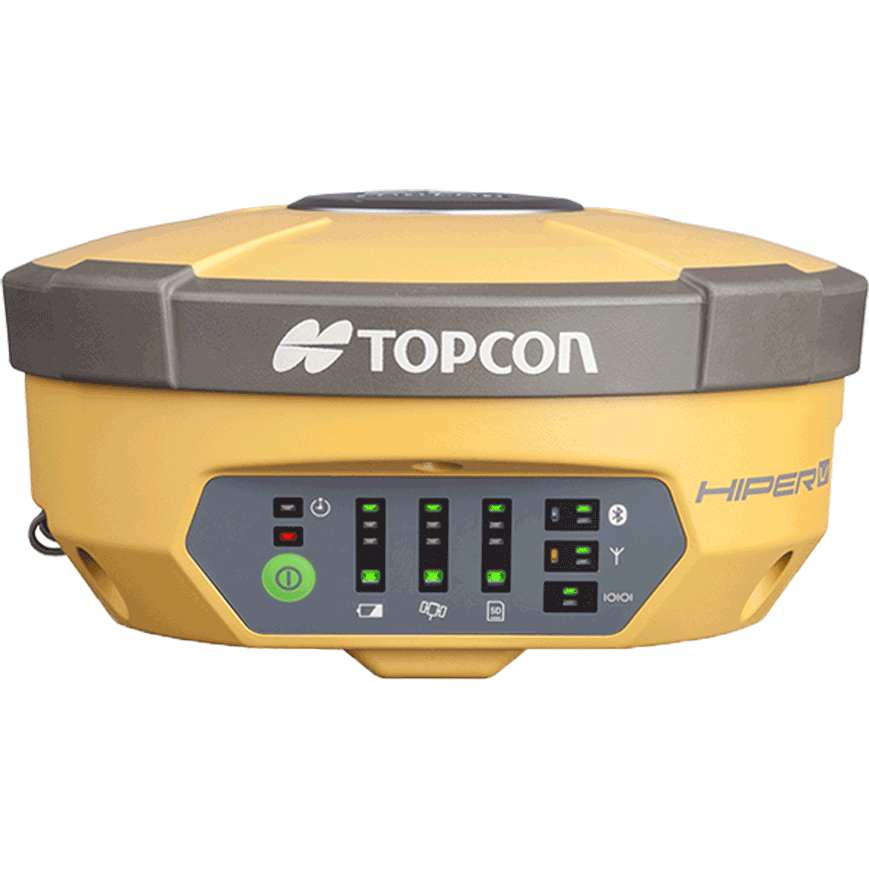
\includegraphics[height=1.4cm]{Chapters/Figures/base_stations/HiPer-V.png} & 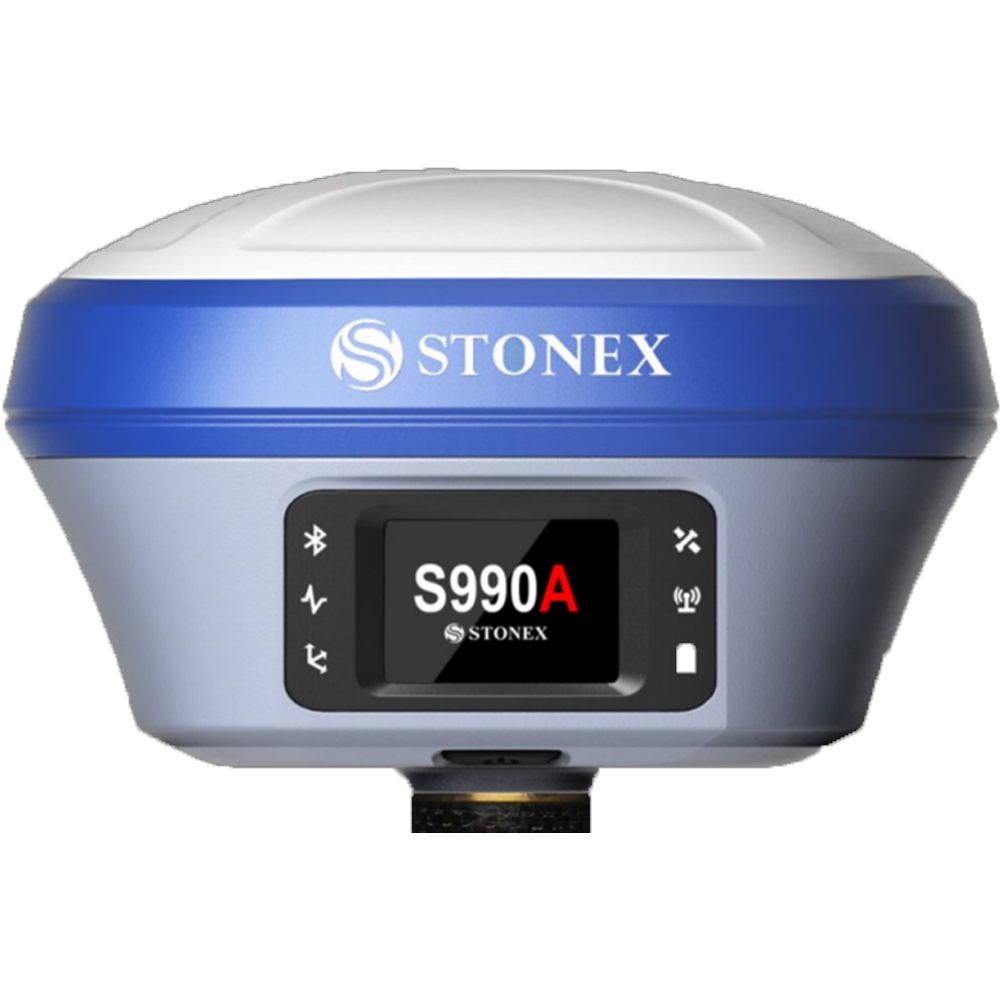
\includegraphics[height=1.4cm]{Chapters/Figures/base_stations/S990A.png}\\
		\bottomrule
	\end{tabular}
\end{table}







% tabela com palavras rodadas:
% \begin{tabular}{m{1em}c}
%     \rotatebox{90}{\textbf{Electrical }}& \makecell{\textbf{Supply} \\ \textbf{Input}\\ \textbf{Battery} \\ \textbf{Autonomy}}\\
% \end{tabular}\\

\newcolumntype{M}[1]{>{\centering\arraybackslash}m{#1}}
\begin{table}[ht]
    \centering
    \captionsetup{justification=centering}
    \caption{Compilation of the most relevant solutions available in the market (as of the date of the present document).}
	\label{tab:currednt_solutions}
    \begin{tabular}{|M{2.5cm}|M{2.5cm}|M{2.5cm}|}
      \hline
      Reconstruction strategy & aa          & bb( \%) \\ \hline
      Classic                 & 3342 voxels & 68 \%   \\ \hline
      VC                      & 4296 voxels & 87 \%   \\ \hline
      V m=7                   & 4745 voxels & 96 \%   \\ \hline
    \end{tabular}
\end{table}

\begin{table}[ht] 
    \centering 
    \begin{tabular}{  >{\raggedright}m{4.5cm}  m{5cm}}      % centered columns (3 columns) 
    \toprule                                   %inserts double horizontal lines 
    Building Block  & Circuits\\  % inserts table heading 
    \midrule\addlinespace[1.5ex]
            Inverting op-amp\\
            (linear amplifier)
            & 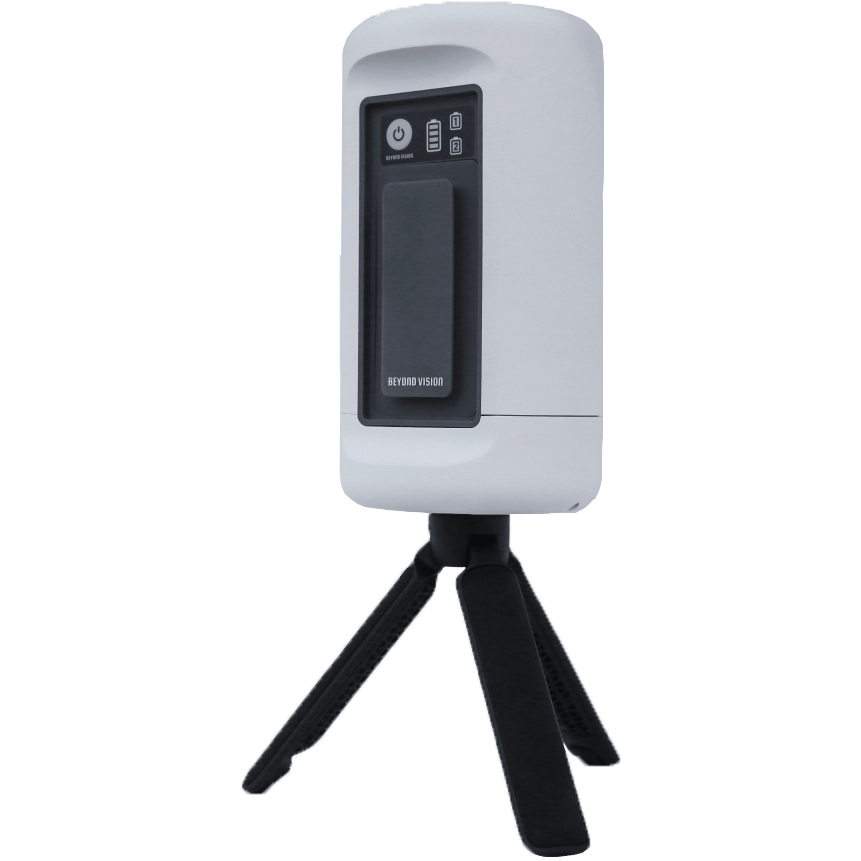
\includegraphics[height=1cm]{Chapters/Figures/base_stations/beRTK_2.png} \\
    \midrule\addlinespace[1.5ex]
            Integrator 
            & 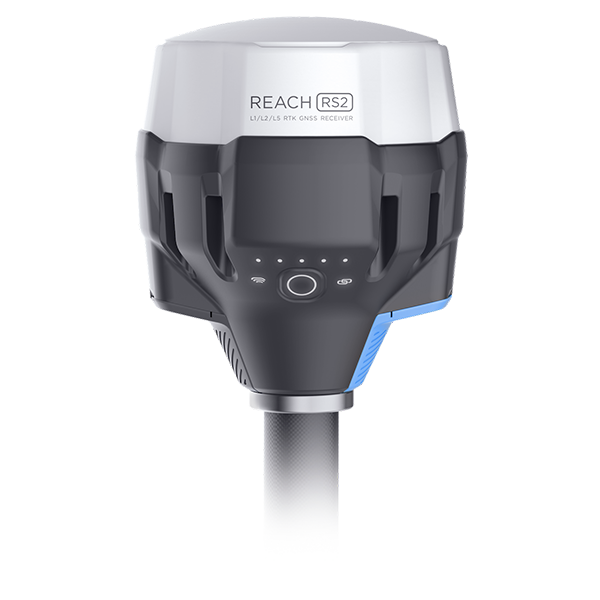
\includegraphics[height=1cm]{Chapters/Figures/base_stations/REACH-RS2.png} \\
    \midrule\addlinespace[1.5ex]
            AC integrator \\ with DC gain
            & 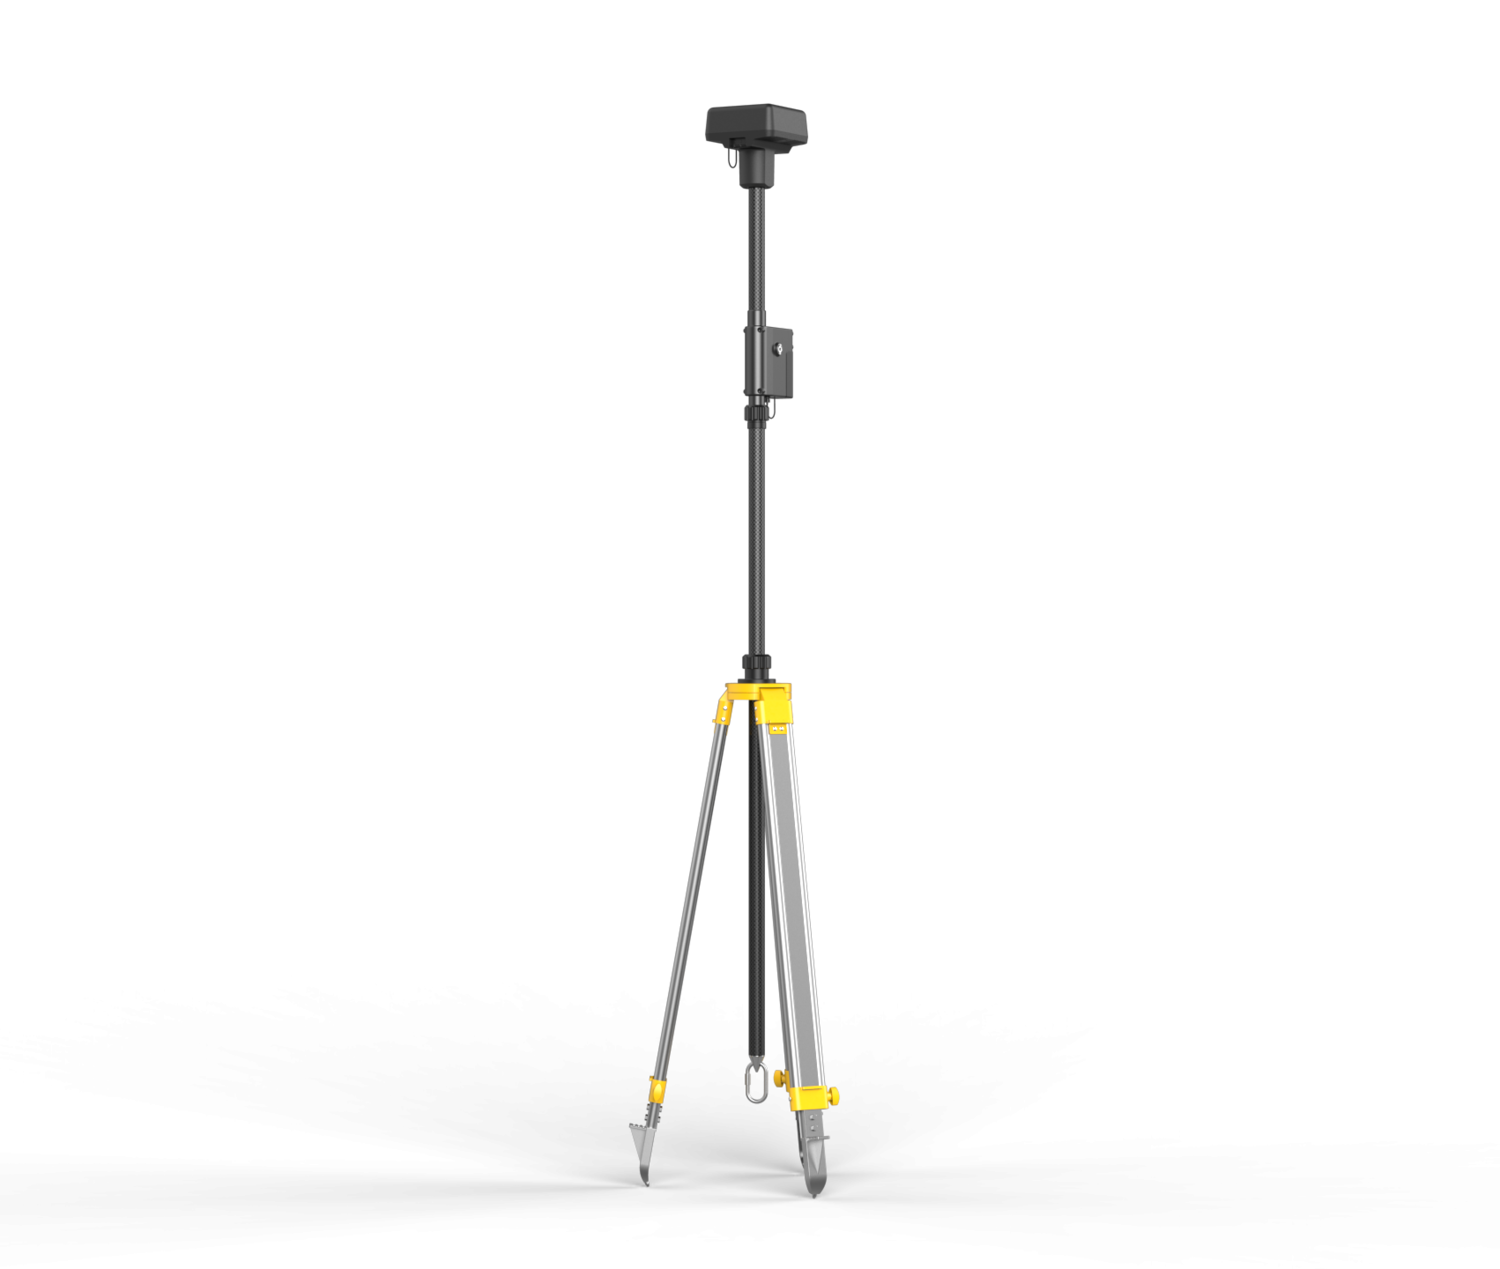
\includegraphics[height=1cm]{Chapters/Figures/base_stations/d-rtk-2.png} \\
    \midrule\addlinespace[1.5ex]
            Differentiator
            & 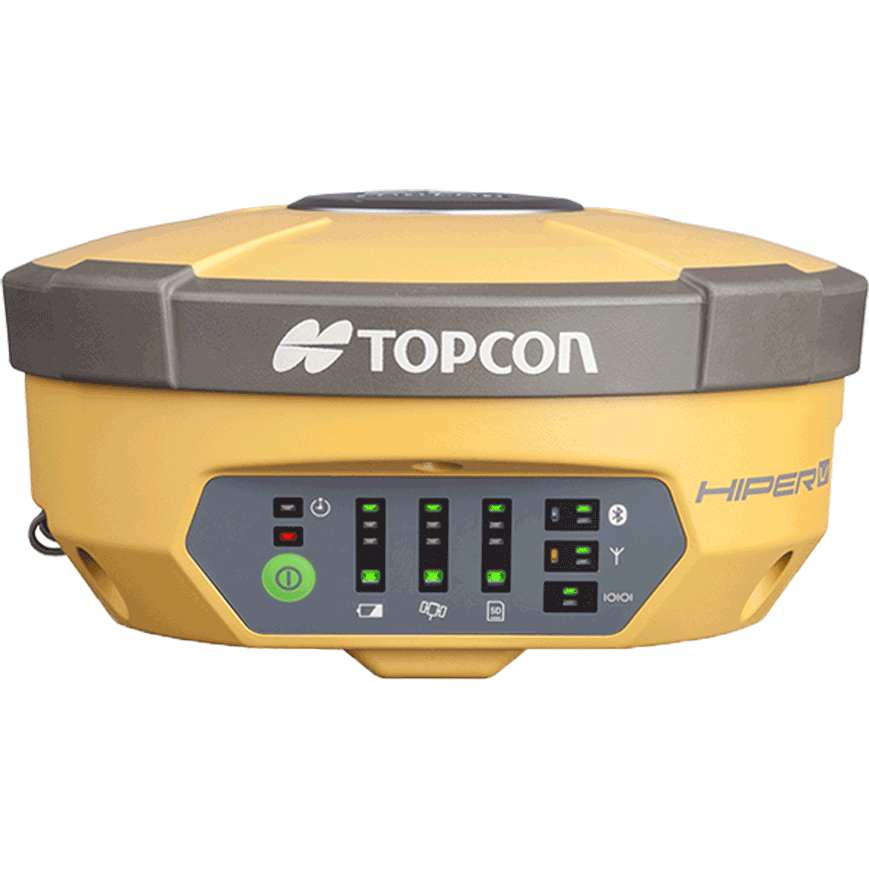
\includegraphics[height=1cm]{Chapters/Figures/base_stations/HiPer-V.png} \\
    \midrule\addlinespace[1.5ex]
            AC differentiator \\ with DC gain
            & 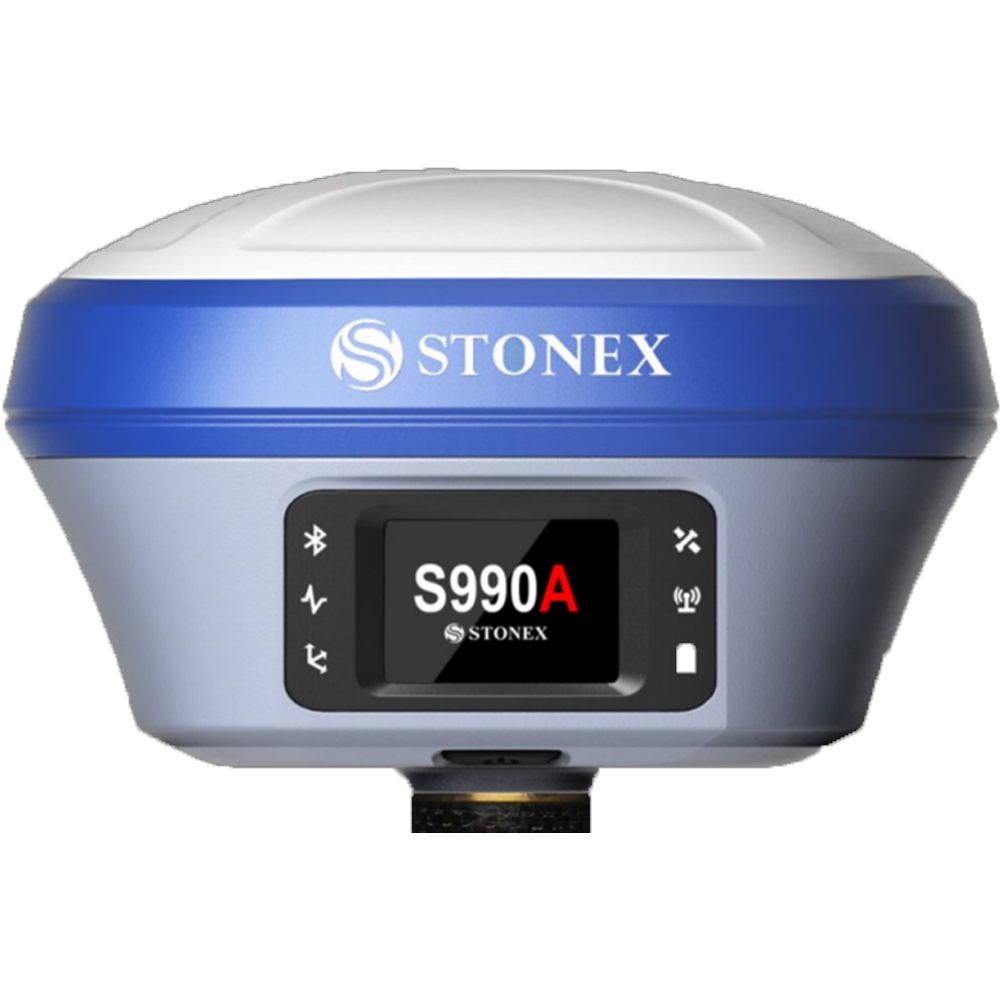
\includegraphics[height=1cm]{Chapters/Figures/base_stations/S990A.png} \\
    \bottomrule
        \end{tabular}
        \caption{A few basic circuit blocks and their frequency response for servo design.}
        \label{table4.2}
\end{table}
